\section{Status and Evaluation}
\label{sec:evaluation}

\subsection{Portability}
We have three proof-of-concept implementations: UDP Sockets, Portals 3.3, and MX.

The Sockets prototype driver opens one SOCK\_DGRAM (UDP) socket per
CCI endpoint, with CCI  providing optional reliability and optional
ordering (UU, RO, RU). 
The Sockets driver multiplexes connections over a single socket.
Enough functions are complete including RMA to allow simple ping pong
tests to exercise the CCI API.

The Portals implementation provides UU, RO, and RU over the portals
interface. Since Portals assumes a reliable interconnect, the
only difference between a CCI UU connection and a RO/RU connection is that we
complete a UU send when we receive the Portals' SEND\_END event which indicates
that the sender's buffer is no longer needed (i.e. the data is on the wire).
For a reliable connection, we report a completion when we get the Portals' ACK
of receipt at the peer.

The MX driver currently only implements UU active messages.  It takes advantage of
MX's unexpected handler to handle all incoming active messages and connection
requests. MX limits the unexpected handler to 1 KB messages which we adopt as the max
send size for this driver. MX send semantics closely mirror those of MPI, so the
completion is returned once the buffer is modifiable (typically once the contents are
copied out to an intermediate buffer). We will implement RU active messages by using
MX's synchronous (rendezvous) send.

\subsection{Performance}
We wrote ping pong applications for Portals, MX, and CCI.  We tested CCI in lock-less
and locking versions, \emph{CCI} and \emph{CCI Thread-Safe} respectively, for active
message ping pong tests. All binaries were compiled with \texttt{-O3} and
\texttt{-fno-builtin}. Each message size is an average of 512K iterations. Typically,
we saw $\pm$10ns variation for messages up to 1 KB.

We evaluated two different native Portals strategies for sending. The first strategy
binds a buffer, puts the buffer, and then unlinks the buffer; we refer to it as
\emph{Portals Bind}. This is the most intuitive strategy and probably the more
commonly used method by developers. The second strategy allocates a intermediate
buffer and binds it once. The application then copies into the bound buffer before
calling Put. We refer to this as \emph{Portals Copy}. Portals Copy performs better
than Portals bind for messages less than 8 KB.

We ran the Portals tests on a Cray XT6 and locked the processes to the same cores for
both tests. The CCI HRT ping pong is about 200-300ns more than the Portals Copy
performance up to 1 KB.  For an eight byte message, for example, CCI's latency is
5.80\us versus 5.56\us for native Portals.  Figures \ref{fig:latency-portals} and
\ref{fig:bw-portals} show latency and bandwidth for active messages up to 8 KB on the Cray
XT6. Figure \ref{fig:latency-rma} shows latency and overhead for RMA messages up to 4
MB.

For MX tests, we used a pair of machines with dual Intel Nehalems and Myri-10G NICs.
Figure \ref{fig:latency-mx} shows CCI overhead of around 60ns without locks and
around 120ns with locks while figure \ref{fig:bw-mx} shows bandwidth for MX, CCI, and
MPI.

\begin{figure}[htbp]
\centering
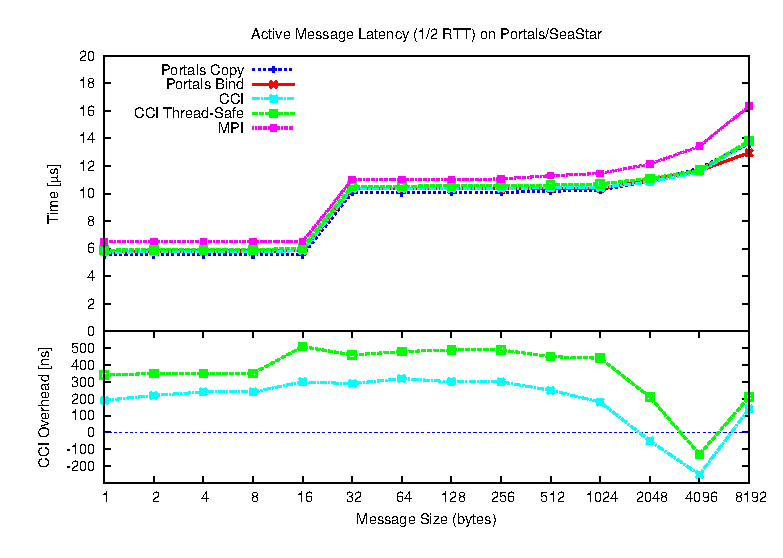
\includegraphics[width=3.45in]{pingpong-latency-portals-overhead-combined.eps}
\caption{Ping pong Latency when using Portals on SeaStar}
\label{fig:latency-portals}
\end{figure}

\begin{figure}[htbp]
\centering
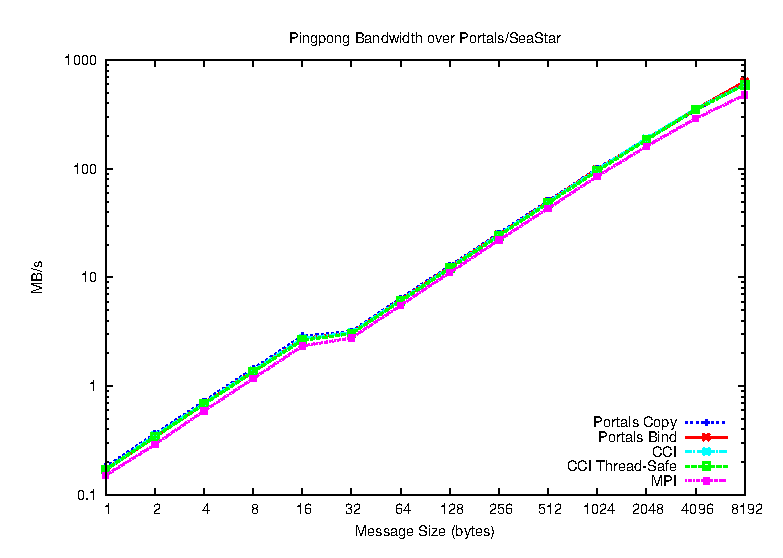
\includegraphics[width=3.45in]{pingpong-bw-portals.eps}
\caption{Ping pong Bandwidth when using Portals on SeaStar}
\label{fig:bw-portals}
\end{figure}

\begin{figure}[htbp]
\centering
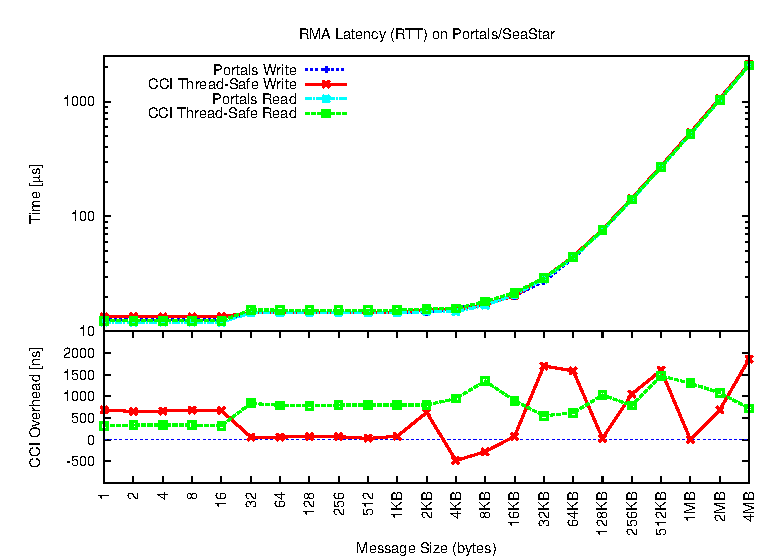
\includegraphics[width=3.45in]{one-sided-latency-portals-overhead.eps}
\caption{RMA Latency when using Portals on SeaStar}
\label{fig:latency-rma}
\end{figure}

\begin{figure}[htbp]
\centering
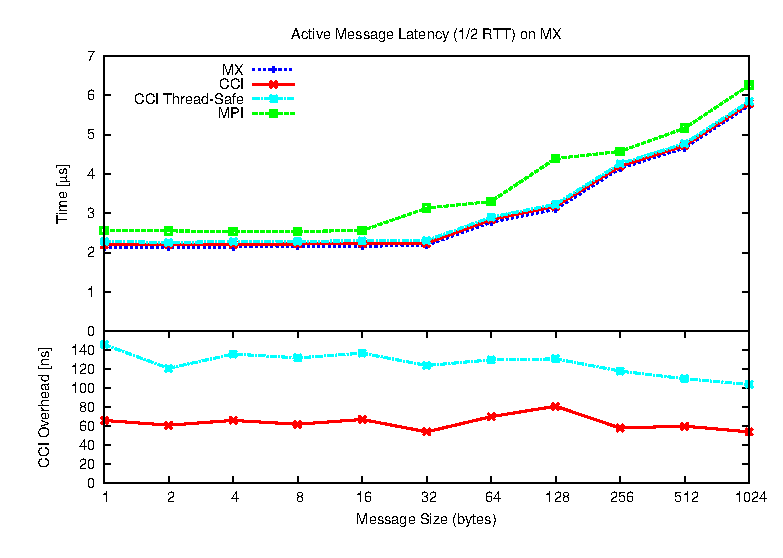
\includegraphics[width=3.45in]{pingpong-latency-mx-overhead-combined.eps}
\caption{Ping pong Latency when using MX}
\label{fig:latency-mx}
\end{figure}

\begin{figure}[htbp]
\centering
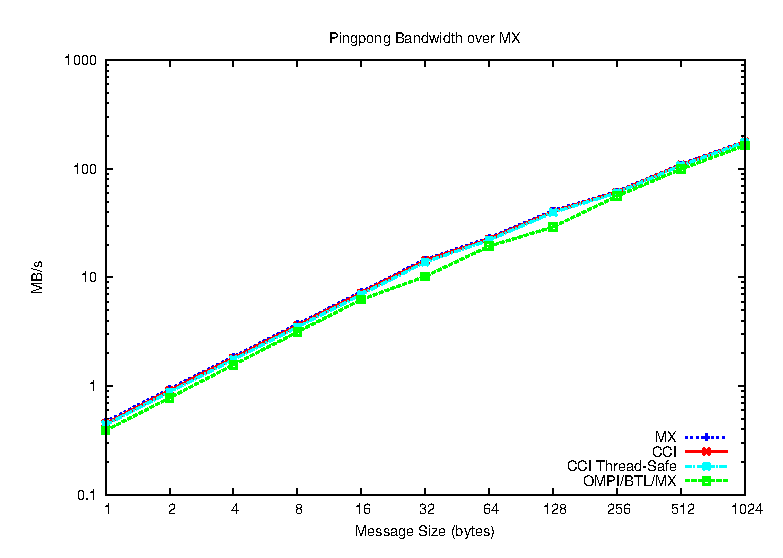
\includegraphics[width=3.45in]{pingpong-bw-mx.eps}
\caption{Ping pong Bandwidth when using MX}
\label{fig:bw-mx}
\end{figure}

\begin{figure}[htbp]
\centering
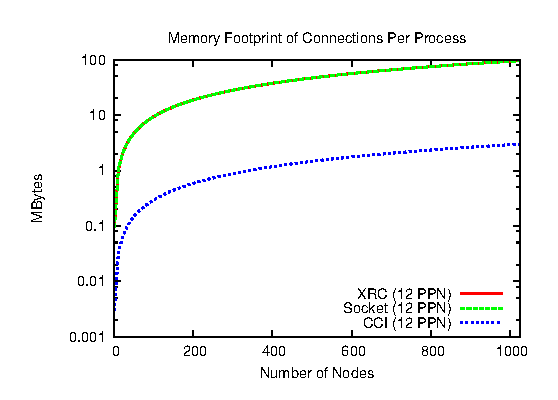
\includegraphics[width=3.45in]{memory_log.eps}
\caption{Memory footprint for connections per process}
\label{fig:memory}
\end{figure}

\subsection{Scalability}
CCI uses connection-oriented semantics with minimal per-connection resources.
For the Portals driver, each connection requires 104 bytes on 64-bit machines
(20 bytes for the public CCI connection struct, 20 bytes for the private CCI
struct, and 64 bytes for the Portals driver connection struct).  The sock driver
needs 140 bytes for each connection.

Figure \ref{fig:memory} illustrates the connection state for
Verbs, BSD Sockets, and CCI. Verbs memory usage scales
linearly~\cite{Shipman:2008:XIS:1431669.1431683} with the number of
connected peers when Reliable Connected (RC) mode. This is
the best case scenario for Verbs. The Sockets usage is derived from
the minimum 4 KB page send and receive buffers and internal state tied
to the connection. 

%% In addition to minimal connection state, CCI, Verbs, and Sockets
%% require additional memory for send/receive buffers. Both CCI and Verbs
%% support a shared memory pool model for send/receive buffers. 

The CCI usage conservatively assumes 256 bytes (assuming alingment padding,
etc.) as used in the UDP driver. Obviously, if CCI is implemented over Verbs,
for example, then this amount is on top of the underlying implementation. In
order to provide support for Verbs hardware (InfiniBand, iWARP, etc.), we intend
to use Verb's Unreliable Datagram (UD) mode to avoid the QP memory usage by
Verb's Reliable Connected (RC) or eXtended Reliable Connected (XRC) modes.

% LocalWords:  DGRAM UU RO RMA ACK XT RTT ns CCI's SeaStar struct alingment UD
% LocalWords:  Datagram QP eXtended
